\documentclass[fontset=windows]{article}
\usepackage[]{ctex}

\title{LSM Tree实验报告}
\author{沈玮杭 519021910766 }
\date{5月26日 2021年}

\usepackage{natbib}
\usepackage{graphicx}
\usepackage{enumitem}
\begin{document}

\maketitle

\section{背景介绍}
LSM Tree (log-structured merge-tree)是一种具有较高写性能的数据存储系统。LSM Tree克服了B+树在写操作时会产生大量随机IO的性能缺陷。相比B+树,它牺牲了一部分读性能,而大大增加了写性能。对于以硬盘为主要存储媒介的大容量数据存储系统,LSM Tree是一个非常合适的存储策略。LSM Tree已在Apache HBase数据库使用,正在工业界推广。

LST Tree主要由三个部分组成:MemTable、Immutable MemTable和SSTable (Sorted String Table)。MemTable是一个跳表,储存在内存中,用于保存最近更新的数据。当MemTable达到设定阈值时,会转化为Immutable MemTable,此时写操作由新的MemTable处理,该Immutable MemTable正在被转化成SSTable储存到磁盘上,这样可以使得在保存过程中的操作不会被阻塞。在本次lab中,由于没有这样的需求,因此Immutable MemTable不是必要的。SSTable是存储在磁盘上的键值对集合。为了加快SSTable的读取,在本次lab建立了索引以及BloomFilter(布隆过滤器)来加速查找。SSTable和LSM Tree的结构如图~\ref{fig:sstable}和图~\ref{fig:lsm}所示。

\begin{figure}[h!]
\centering
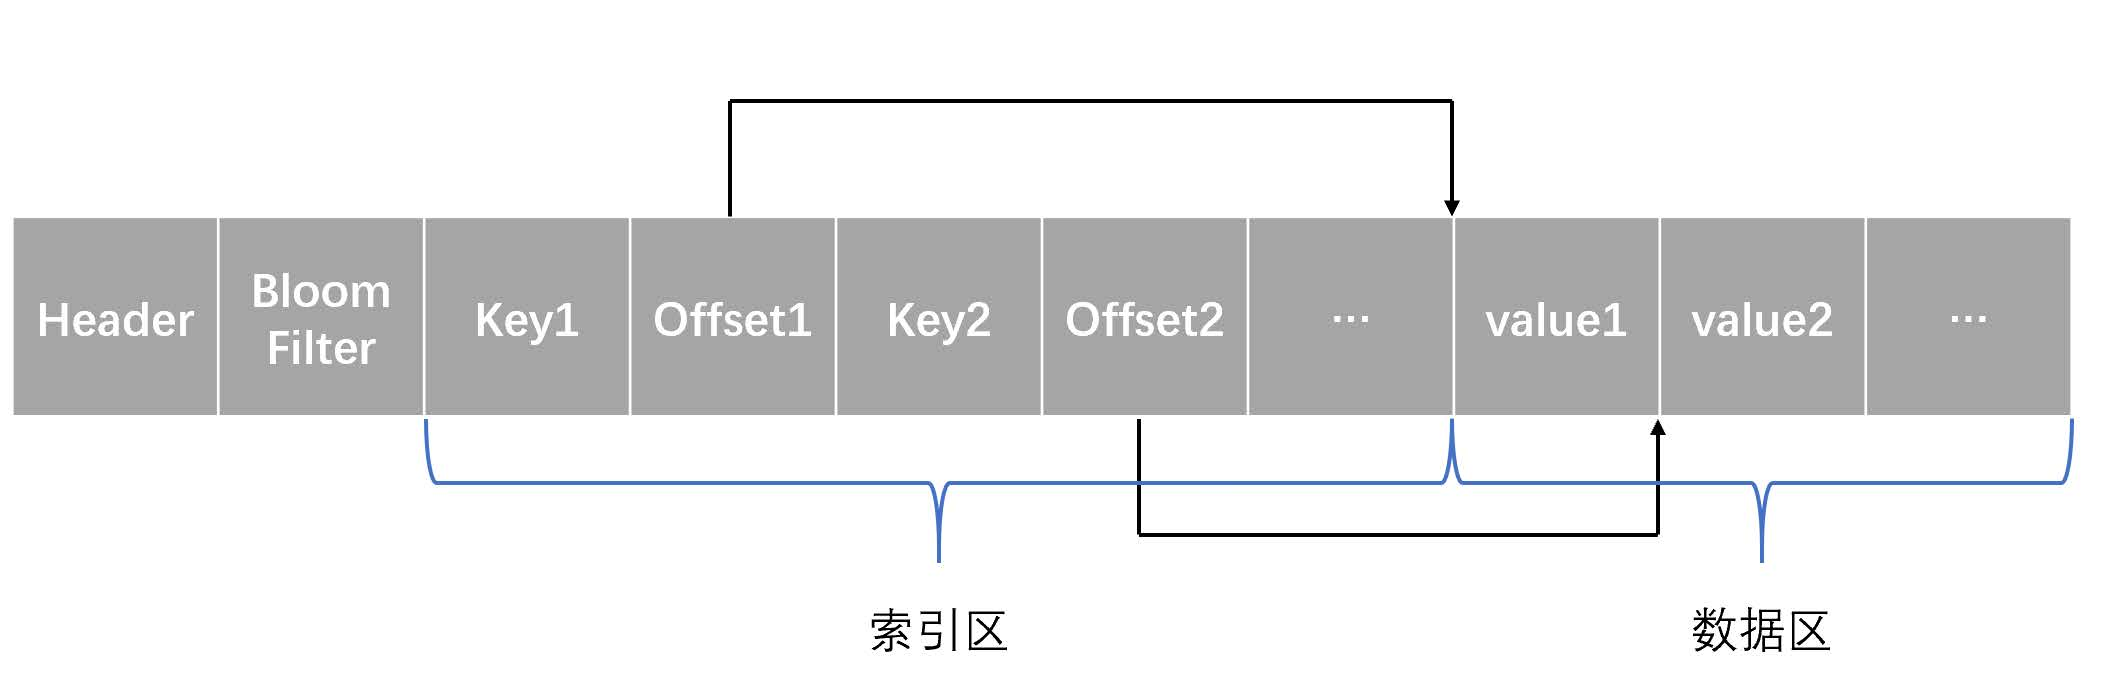
\includegraphics[scale=0.8]{sstable}
\caption{SSTable结构}
\label{fig:sstable}
\end{figure}

\begin{figure}[h!]
\centering
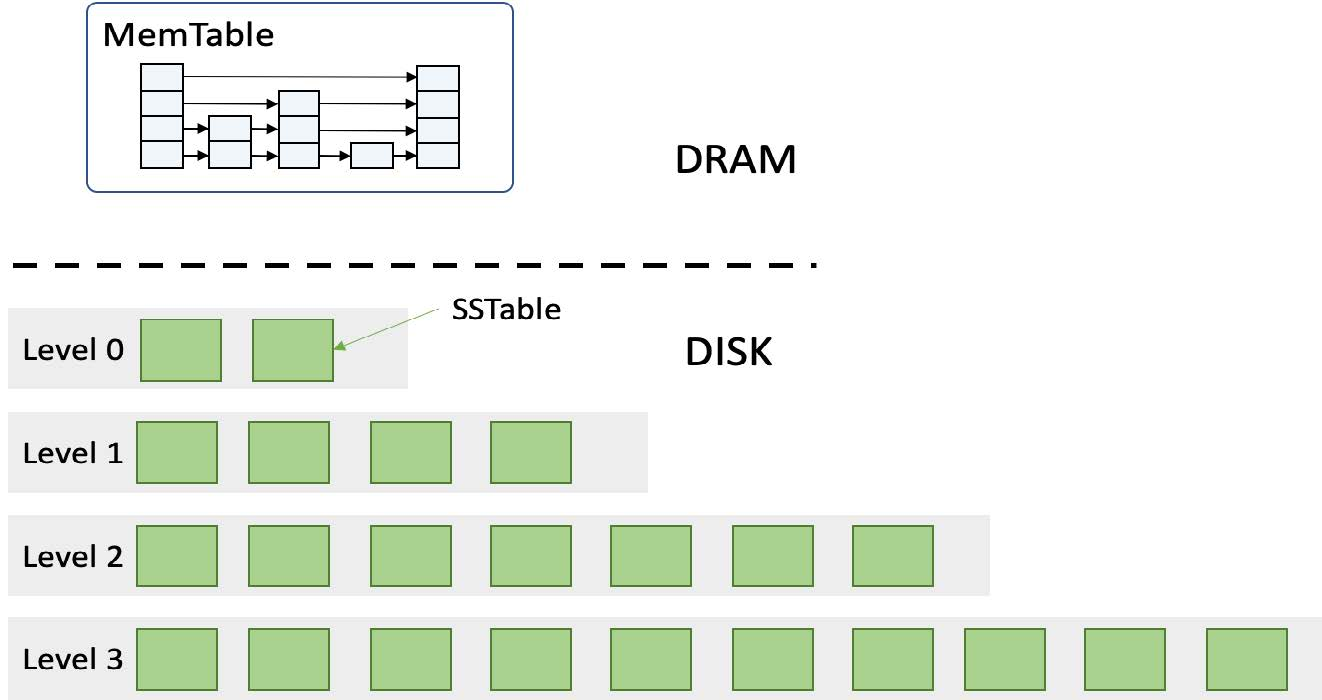
\includegraphics[scale=1]{lsm}
\caption{LSM Tree结构}
\label{fig:lsm}
\end{figure}

\section{挑战}
内存中的SkipList和读写SSTable都很好实现,最具挑战性的是SSTable的合并,需要慎重地分析每一种情况,
仔细地检查每一行代码才能保证正确。

在选择SSTable进行合并时需要特别谨慎,我一开始并没有考虑上一层的SSTable时间戳相同的情况,只是选择了固定数量的时间戳最大的SSTable。结果导致在特殊情况下会出现bug:如上一层有10个时间戳为5的SSTable,从中选出了5个与下层合并,若下层与其合并的SSTable中有若干个与上层剩余的5个时间戳为5的SSTable有交集时,由于此次合并生成的时间戳是最大的,在下一次合并时,下一层中旧的值可能会覆盖上一层中新的值,会导致错误。这个问题在文档中没有细说,也很难发现,耗费了我很多时间。


\section{测试}
该部分对LSM Tree的性能进行了测试,主要分析了PUT、GET和DEL操作的吞吐量和时延,并修改了代码逻辑来对比分析内存中BloomFilter和索引缓存对GET性能的影响。


\subsection{性能测试}

\subsubsection{预期结果}
由于没有使用多线程加速,三种操作的吞吐量和时延应为倒数关系。由于DEL操作要返回store中是否存在,所以要先做一次GET,再插入一个``\textasciitilde DELETED\textasciitilde '',因此DEL操作时延可能会比GET略高。而PUT操作可能会触发合并,而一次合并有较大的性能开销,因此在持续PUT时会有若干次时延相当高。又因为DEL插入的字符串很小,只有9个字节,很少会触发合并,因此字符串很长的PUT操作时延会显著高于DEL。

BloomFliter可以提前判断SSTable中是否有查询的key,可以避免无用的查找,因此会提高很多GET性能。由于磁盘的速度比内存慢很多个数量级,在内存中缓存index可以显著地加快查找的速度。

\subsubsection{常规分析}


\begin{enumerate}
    \item GET、PUT、DEL操作的延迟:
    
    测试GET使用随机的key进行插入,插入的Value大小为10000字节。测试PUT和DEL使用随机的key,并且该key在store中不存在的概率约为0.2,以模拟真实的使用场景。每种操作的测试包含100、1000、10000个条目的三种规模的测试。由于篇幅原因,且代表性没有10000条目的强,100、1000条目的时延图就不在此给出。
    
    在100条目规模的测试中,由于MemTable未达到阈值,故三种操作时延均很理想:GET操作平均时延为$0.76 \mu s$,PUT操作平均时延为$6.56 \mu s$,DEL操作平均时延为$0.65 \mu s$。
    
    在1000条目规模的测试中,由于MemTable达到阈值,会产生磁盘读写,故时延变大:GET操作平均时延为$25.74 \mu s$,PUT操作平均时延为$34.08 \mu s$,DEL操作平均时延为$17.76 \mu s$。
    
    在10000条目规模的测试中,时延进一步变大:GET操作平均时延为$33.34 \mu s$,PUT操作平均时延为$173.19 \mu s$,DEL操作平均时延为$23.00 \mu s$。
    
    从图~\ref{fig:get_with_cache}可以看出,10000次GET操作中,大多数时延分布在$35.4 \mu s$到$40.8 \mu s$和$0.3 \mu s$到$3.0 \mu s$间,其中后者是直接在MemTable中直接访问的时延。
    
    图~\ref{fig:put_with_cache}中的尖峰表示此处触发了一次合并,可以发现合并操作非常耗时,因此也导致了PUT操作平均时延变长。
    
    与预期结果不同,DEL操作反而要略快于GET操作。从图图~\ref{fig:del_with_cache}中可以看出,在MemTable命中的次数增加了,猜测可能是由于一次DEL操作至多插入9个字节,数据量很小,所以MemTable所能容纳的条目变多了。
    
\begin{figure}[h!]
\centering
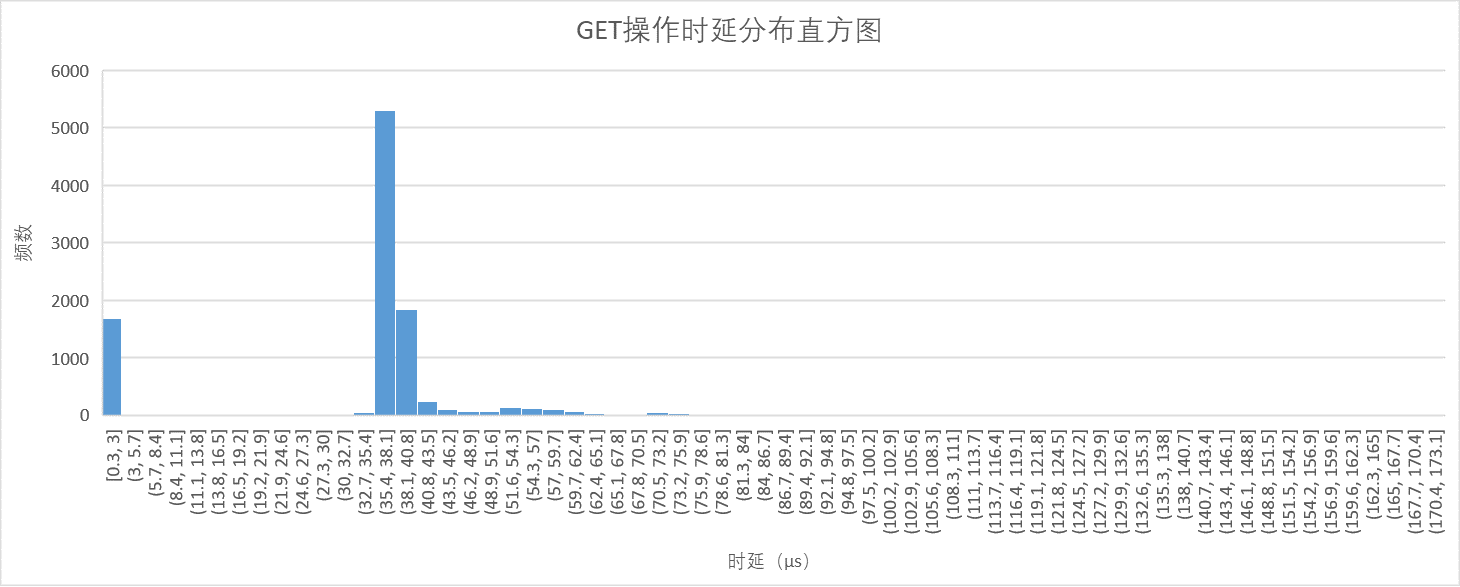
\includegraphics[scale=0.5]{get_with_cache}
\caption{带缓存的10000次GET操作时延分布直方图}
\label{fig:get_with_cache}
\end{figure}

\begin{figure}[h!]
\centering
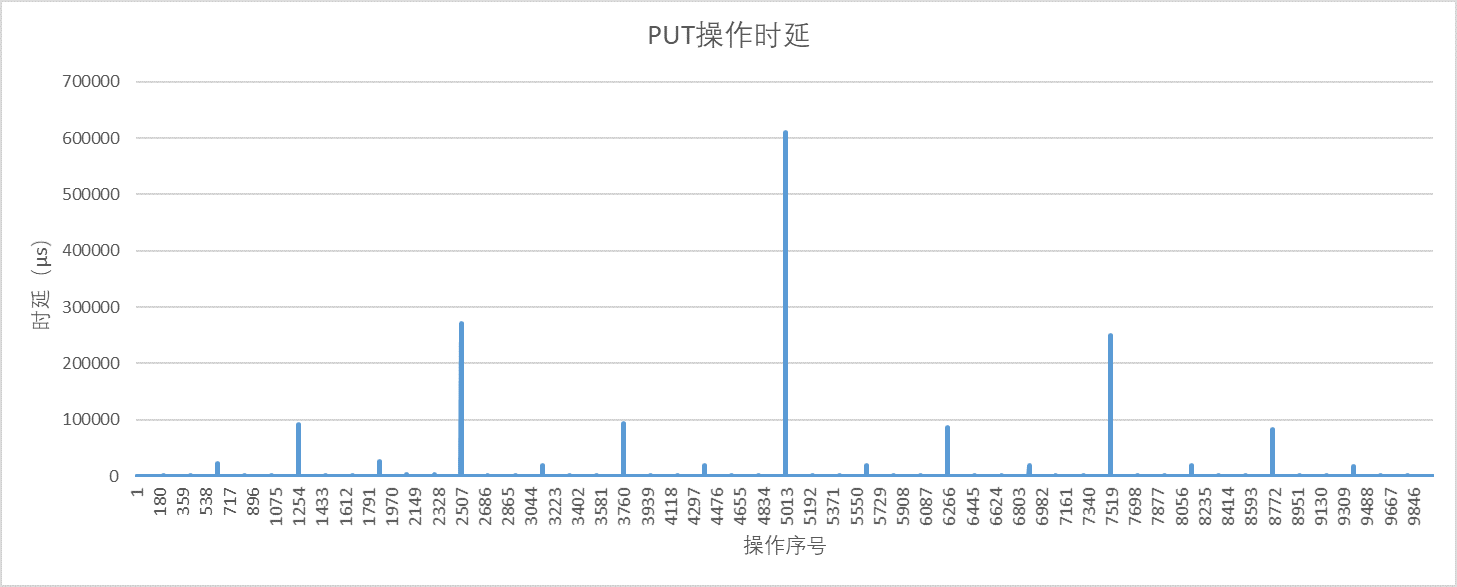
\includegraphics[scale=0.5]{put_with_cache}
\caption{带缓存的10000次PUT操作时延}
\label{fig:put_with_cache}
\end{figure}

\begin{figure}[h!]
\centering
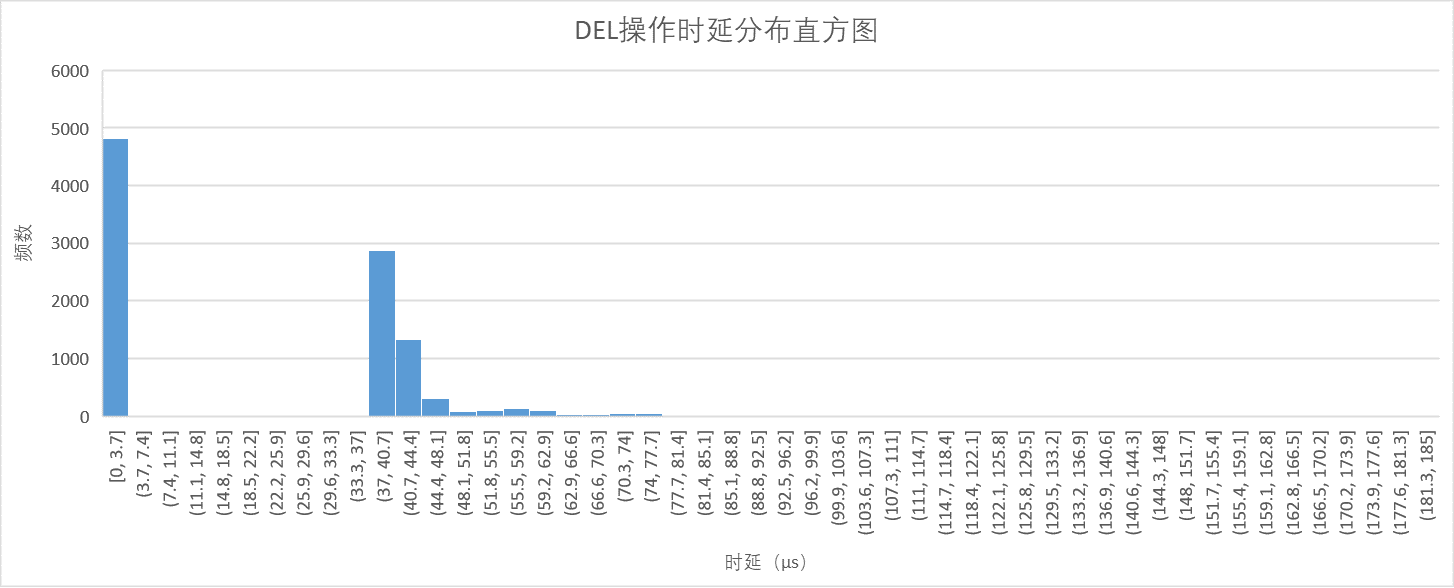
\includegraphics[scale=0.5]{del_with_cache}
\caption{带缓存的10000次DEL操作时延分布直方图}
\label{fig:del_with_cache}
\end{figure}
    
    \item GET、PUT、DEL操作的吞吐:
    
    经计算:
    
    在100条目规模的测试中,GET操作吞吐量为1315789IOPS,PUT操作吞吐量为152439IOPS,DEL操作吞吐量为1538461IOPS。
    
    在1000条目规模的测试中,GET操作吞吐量为38850IOPS,PUT操作吞吐量为29342IOPS,DEL操作吞吐量为56306IOPS。
    
    在10000条目规模的测试中,GET操作吞吐量为29994IOPS,PUT操作吞吐量为5774IOPS,DEL操作吞吐量为43478IOPS。
\end{enumerate}


\subsubsection{索引缓存与Bloom Filter的效果测试}
本次lab对比了以下三种情况GET操作的平均时延:
\begin{enumerate}
    \item 内存中没有缓存SSTable的任何信息,从磁盘中访问SSTable的索引,在找到offset之后读取数据:
    
	在100条目规模的测试中,GET操作平均时延为$0.60 \mu s$。在1000条目规模的测试中GET操作平均时延为$444.53 \mu s$。在10000条目规模的测试中,GET操作平均时延为$1290.85 \mu s$。
    
    \item 内存中只缓存了SSTable的索引信息,通过二分查找从SSTable的索引中找到offset,并在磁盘中读取对应的值:
    
    在100条目规模的测试中,GET操作平均时延为$1.38 \mu s$。在1000条目规模的测试中GET操作平均时延为$32.26 \mu s$。在10000条目规模的测试中,GET操作平均时延为$40.55 \mu s$。
    
\begin{figure}[h!]
\centering
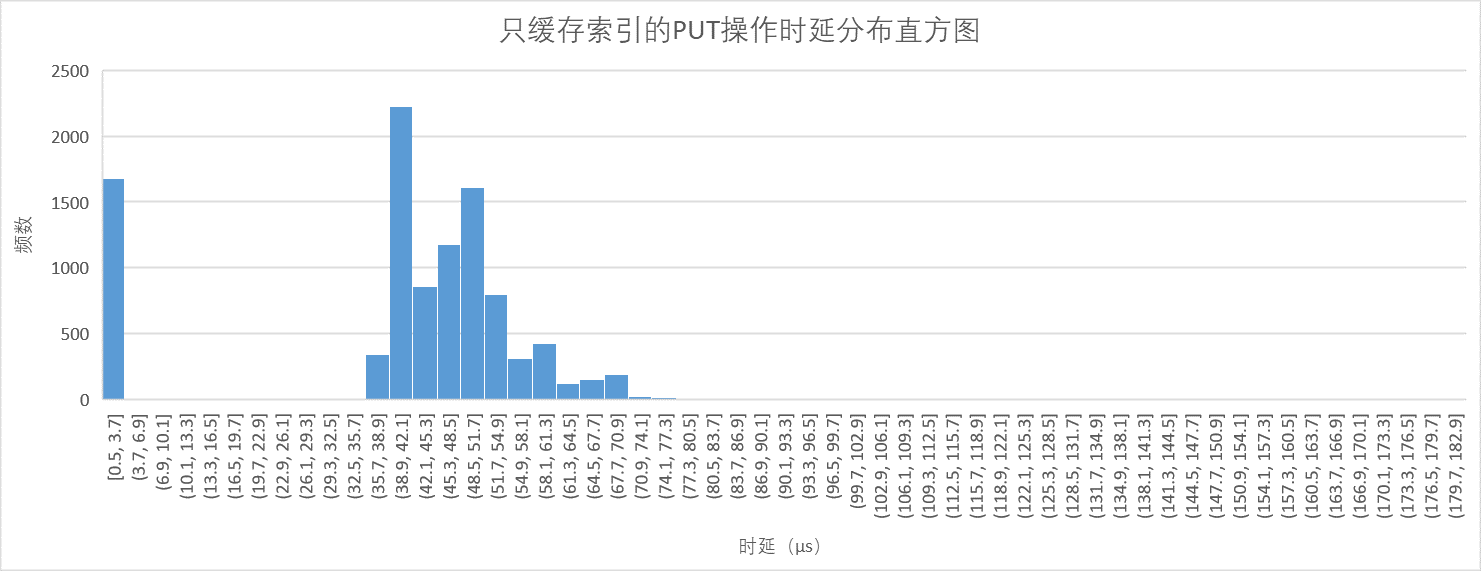
\includegraphics[scale=0.5]{put_part_cache}
\caption{只缓存索引的10000次PUT操作时延分布直方图}
\label{fig:put_part_cache}
\end{figure}
    
    \item 内存中缓存SSTable的Bloom Filter和索引,先通过Bloom Filter判断一个键值是否可能在一个SSTable中,如果存在再利用二分查找,否则直接查看下一个SSTable的索引:
    
    在100条目规模的测试中,GET操作平均时延为$0.76 \mu s$。在1000条目规模的测试中GET操作平均时延为$25.74 \mu s$。在10000条目规模的测试中,GET操作平均时延为$33.34 \mu s$。
    
\begin{figure}[h!]
\centering
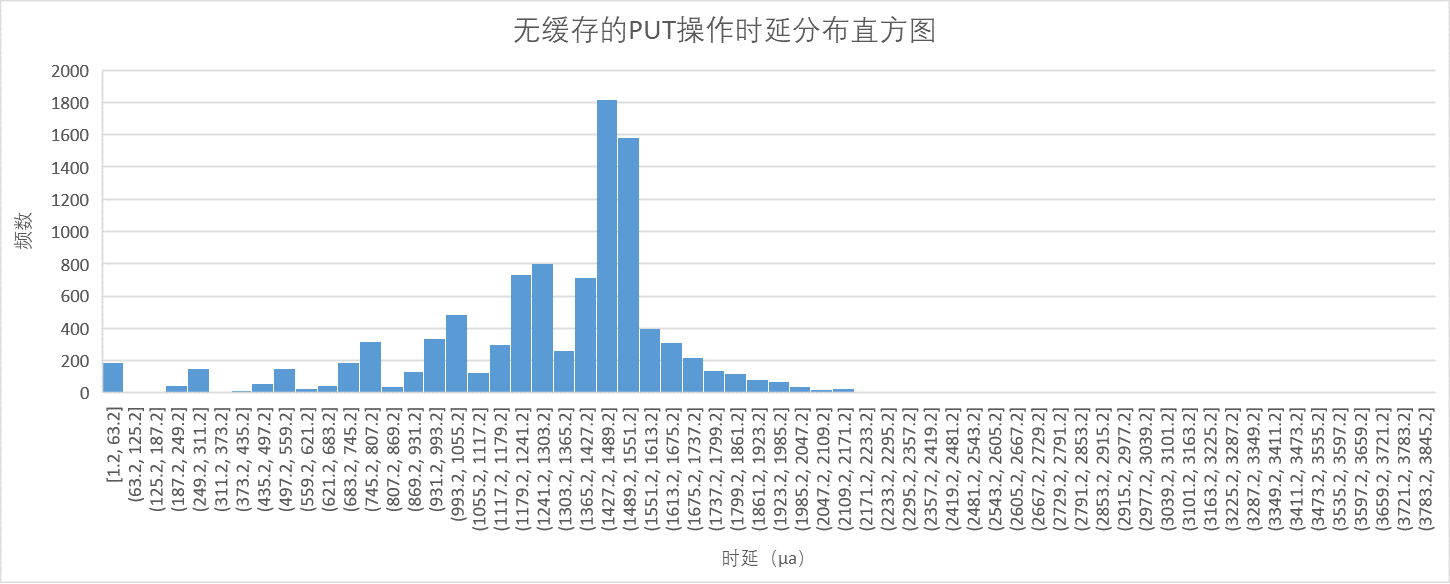
\includegraphics[scale=0.5]{put_no_cache}
\caption{无缓存的10000次PUT操作时延分布直方图}
\label{fig:put_no_cache}
\end{figure} 

从结果可以看出BloomFilter对性能提升有一定作用,而缓存索引由于可以大大减少对磁盘的随机读写,因此可以显著地提高LSM Tree的性能。由于篇幅原因,且代表性没有10000条目的强,100、1000条目的时延图就不在此给出。
    
\end{enumerate}

\subsubsection{Compaction的影响}
本次lab统计了不断插入数据的情况下,统计每秒钟处理的PUT请求个数(即吞吐量),并绘制其随时间的变化图,如图~\ref{fig:put_iops}所示。

\begin{figure}[h!]
\centering
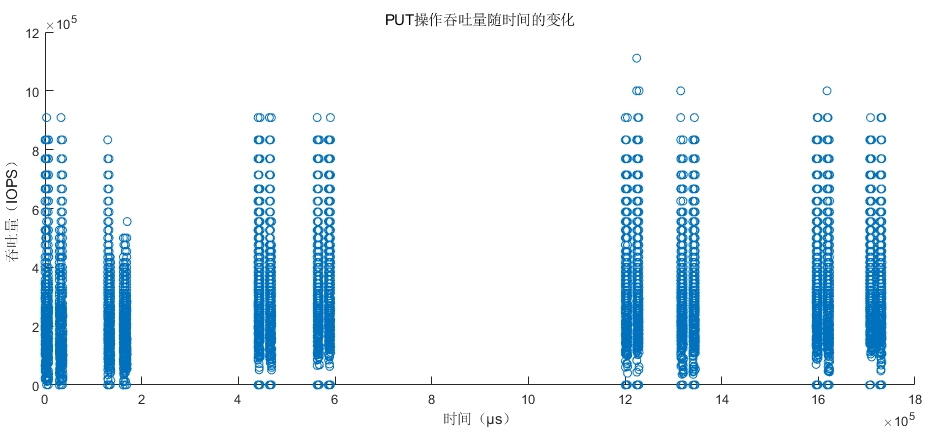
\includegraphics[scale=0.5]{put_iops}
\caption{10000次PUT操作吞吐量随时间的变化}
\label{fig:put_iops}
\end{figure}

插入的数据为10000个Key随机Value大小为10000的键值对。图中间的空白表示在这段时间内都在执行合并,没有数据插入,因此没有吞吐。图~\ref{fig:put_with_cache}也很好地展示了合并操作的影响,每一次合并表现为一次较长的时延,且合并层数越深,合并时间越长。

\section{结论}

通过常规分析,可以发现DEL操作略快于GET操作,并显著快于PUT操作。通过对比有无缓存的情况,可以得出BloomFilter对GET操作性能提升较小,而索引缓存对GET性能的提升很大。对Compaction的分析表明,PUT操作慢的主要原因是合并时间很长。一般情况下PUT操作很快,而若需要合并,则操作的时延会高几个数量级。

LSM Tree是一个根据计算机各存储结构设计的键值对存储系统,既通过SSTable和索引缓存的方式规避了磁盘随机读写慢的问题,同时也通过MemTable的方式充分发挥了内存高速读写的优势。LSM Tree也很好地利用了局部性原则,将最频繁使用的数据放在最快的地方,同时获得了近与内存的速度和近于磁盘的大容量。LSM Tree的设计思路很巧妙,也非常值得我们学习。同时,这也告诉我们在设计系统时要充分考虑和利用计算机体系结构的特性和使用场景。

在本次lab中,我的代码能力也有所提高,也明白了动手之前要先想清楚,然后再写代码。


\end{document}
